% created by command line:
%   tmp/petsc2tikz.py --labelnodes --nodesize 1.0 --dirichletsize 3.0 --nodeoffset -0.5 --scale 0.63 tmp/blob1 -o tmp/blob1_nodenum.tikz
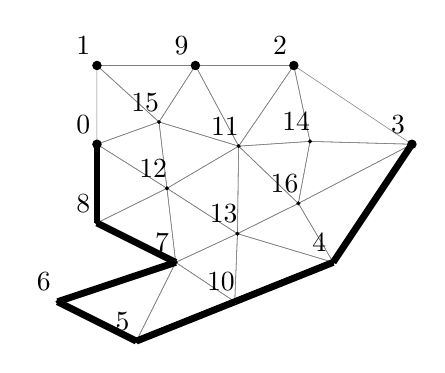
\begin{tikzpicture}[scale=0.5]
  \draw[gray,very thin] (2.000000,-3.000000) -- (3.500000,-4.000000) -- (1.000000,-5.000000) -- (2.000000,-3.000000) ;
  \draw[gray,very thin] (5.000000,2.000000) -- (3.598633,-0.048909) -- (2.500000,2.000000) -- (5.000000,2.000000) ;
  \draw[gray,very thin] (5.000000,2.000000) -- (8.000000,0.000000) -- (5.410836,0.072145) -- (5.000000,2.000000) ;
  \draw[gray,very thin] (6.000000,-3.000000) -- (3.500000,-4.000000) -- (3.567839,-2.271643) -- (6.000000,-3.000000) ;
  \draw[gray,very thin] (2.500000,2.000000) -- (3.598633,-0.048909) -- (1.575312,0.566253) -- (2.500000,2.000000) ;
  \draw[gray,very thin] (5.410836,0.072145) -- (8.000000,0.000000) -- (5.115191,-1.502985) -- (5.410836,0.072145) ;
  \draw[gray,very thin] (2.000000,-3.000000) -- (0.000000,-2.000000) -- (1.777927,-1.119826) -- (2.000000,-3.000000) ;
  \draw[gray,very thin] (8.000000,0.000000) -- (6.000000,-3.000000) -- (5.115191,-1.502985) -- (8.000000,0.000000) ;
  \draw[gray,very thin] (3.598633,-0.048909) -- (1.777927,-1.119826) -- (1.575312,0.566253) -- (3.598633,-0.048909) ;
  \draw[gray,very thin] (2.000000,-3.000000) -- (1.777927,-1.119826) -- (3.567839,-2.271643) -- (2.000000,-3.000000) ;
  \draw[gray,very thin] (5.000000,2.000000) -- (5.410836,0.072145) -- (3.598633,-0.048909) -- (5.000000,2.000000) ;
  \draw[gray,very thin] (0.000000,0.000000) -- (1.777927,-1.119826) -- (0.000000,-2.000000) -- (0.000000,0.000000) ;
  \draw[gray,very thin] (3.598633,-0.048909) -- (3.567839,-2.271643) -- (1.777927,-1.119826) -- (3.598633,-0.048909) ;
  \draw[gray,very thin] (0.000000,2.000000) -- (2.500000,2.000000) -- (1.575312,0.566253) -- (0.000000,2.000000) ;
  \draw[gray,very thin] (6.000000,-3.000000) -- (3.567839,-2.271643) -- (5.115191,-1.502985) -- (6.000000,-3.000000) ;
  \draw[gray,very thin] (0.000000,0.000000) -- (0.000000,2.000000) -- (1.575312,0.566253) -- (0.000000,0.000000) ;
  \draw[gray,very thin] (2.000000,-3.000000) -- (3.567839,-2.271643) -- (3.500000,-4.000000) -- (2.000000,-3.000000) ;
  \draw[gray,very thin] (0.000000,0.000000) -- (1.575312,0.566253) -- (1.777927,-1.119826) -- (0.000000,0.000000) ;
  \draw[gray,very thin] (3.598633,-0.048909) -- (5.410836,0.072145) -- (5.115191,-1.502985) -- (3.598633,-0.048909) ;
  \draw[gray,very thin] (3.598633,-0.048909) -- (5.115191,-1.502985) -- (3.567839,-2.271643) -- (3.598633,-0.048909) ;
  \draw[gray,very thin] (2.000000,-3.000000) -- (1.000000,-5.000000) -- (-1.000000,-4.000000) -- (2.000000,-3.000000) ;
  \filldraw (0.000000,0.000000) circle (3.000000pt);
  \draw (-0.350000,0.500000) node {$0$};
  \filldraw (0.000000,2.000000) circle (3.000000pt);
  \draw (-0.350000,2.500000) node {$1$};
  \filldraw (5.000000,2.000000) circle (3.000000pt);
  \draw (4.650000,2.500000) node {$2$};
  \filldraw (8.000000,0.000000) circle (3.000000pt);
  \draw (7.650000,0.500000) node {$3$};
  \filldraw (6.000000,-3.000000) circle (1.000000pt);
  \draw (5.650000,-2.500000) node {$4$};
  \filldraw (1.000000,-5.000000) circle (1.000000pt);
  \draw (0.650000,-4.500000) node {$5$};
  \filldraw (-1.000000,-4.000000) circle (1.000000pt);
  \draw (-1.350000,-3.500000) node {$6$};
  \filldraw (2.000000,-3.000000) circle (1.000000pt);
  \draw (1.650000,-2.500000) node {$7$};
  \filldraw (0.000000,-2.000000) circle (1.000000pt);
  \draw (-0.350000,-1.500000) node {$8$};
  \filldraw (2.500000,2.000000) circle (3.000000pt);
  \draw (2.150000,2.500000) node {$9$};
  \filldraw (3.500000,-4.000000) circle (1.000000pt);
  \draw (3.150000,-3.500000) node {$10$};
  \filldraw (3.598633,-0.048909) circle (1.000000pt);
  \draw (3.248633,0.451091) node {$11$};
  \filldraw (1.777927,-1.119826) circle (1.000000pt);
  \draw (1.427927,-0.619826) node {$12$};
  \filldraw (3.567839,-2.271643) circle (1.000000pt);
  \draw (3.217839,-1.771643) node {$13$};
  \filldraw (5.410836,0.072145) circle (1.000000pt);
  \draw (5.060836,0.572145) node {$14$};
  \filldraw (1.575312,0.566253) circle (1.000000pt);
  \draw (1.225312,1.066253) node {$15$};
  \filldraw (5.115191,-1.502985) circle (1.000000pt);
  \draw (4.765191,-1.002985) node {$16$};
  \draw[line width=2.500000pt] (8.000000,0.000000) -- (6.000000,-3.000000);
  \draw[line width=2.500000pt] (6.000000,-3.000000) -- (3.500000,-4.000000);
  \draw[line width=2.500000pt] (3.500000,-4.000000) -- (1.000000,-5.000000);
  \draw[line width=2.500000pt] (1.000000,-5.000000) -- (-1.000000,-4.000000);
  \draw[line width=2.500000pt] (-1.000000,-4.000000) -- (2.000000,-3.000000);
  \draw[line width=2.500000pt] (2.000000,-3.000000) -- (0.000000,-2.000000);
  \draw[line width=2.500000pt] (0.000000,-2.000000) -- (0.000000,0.000000);
\end{tikzpicture}
